% Copyright (c) 2013 Benky
% This program is made available under the terms of the MIT License.
\documentclass{article}
\usepackage{tikz}
\usepackage{mathpazo}
\usepackage[top=50mm,left=10mm,right=0mm,bottom=0mm,a1paper]{geometry}
\usepackage{verbatim}


\tikzset{300mT/.pic={
    \draw[line width=4mm] (-6mm, -6mm) -- (6mm, 6mm);
    \draw[line width=4mm] (-6mm, 6mm) -- (6mm, -6mm);
    \draw[line width=3mm] (0in, 0in) circle (25mm); % X
    \draw[line width=3mm] (0in, 0in) circle (59mm); % 10
    \draw[line width=3mm] (0in, 0in) circle (109mm);% 9

    \node[scale=3.0] at (0mm, 42mm) {\large \textbf{10}};
    \node[scale=3.0] at (0mm, -42mm) {\large \textbf{10}};
    \node[scale=3.0] at (42mm, 0mm) {\large \textbf{10}};
    \node[scale=3.0] at (-42mm, 0mm) {\large \textbf{10}};

    \node[scale=7.0] at (0mm, 79.5mm) {\large \textbf{9}};
    \node[scale=7.0] at (0mm, -79.5mm) {\large \textbf{9}};
    \node[scale=7.0] at (79.5mm, 0mm) {\large \textbf{9}};
    \node[scale=7.0] at (-79.5mm, 0mm) {\large \textbf{9}};
}
}


\begin{document}

% Precision target - 300m
\begin{center}
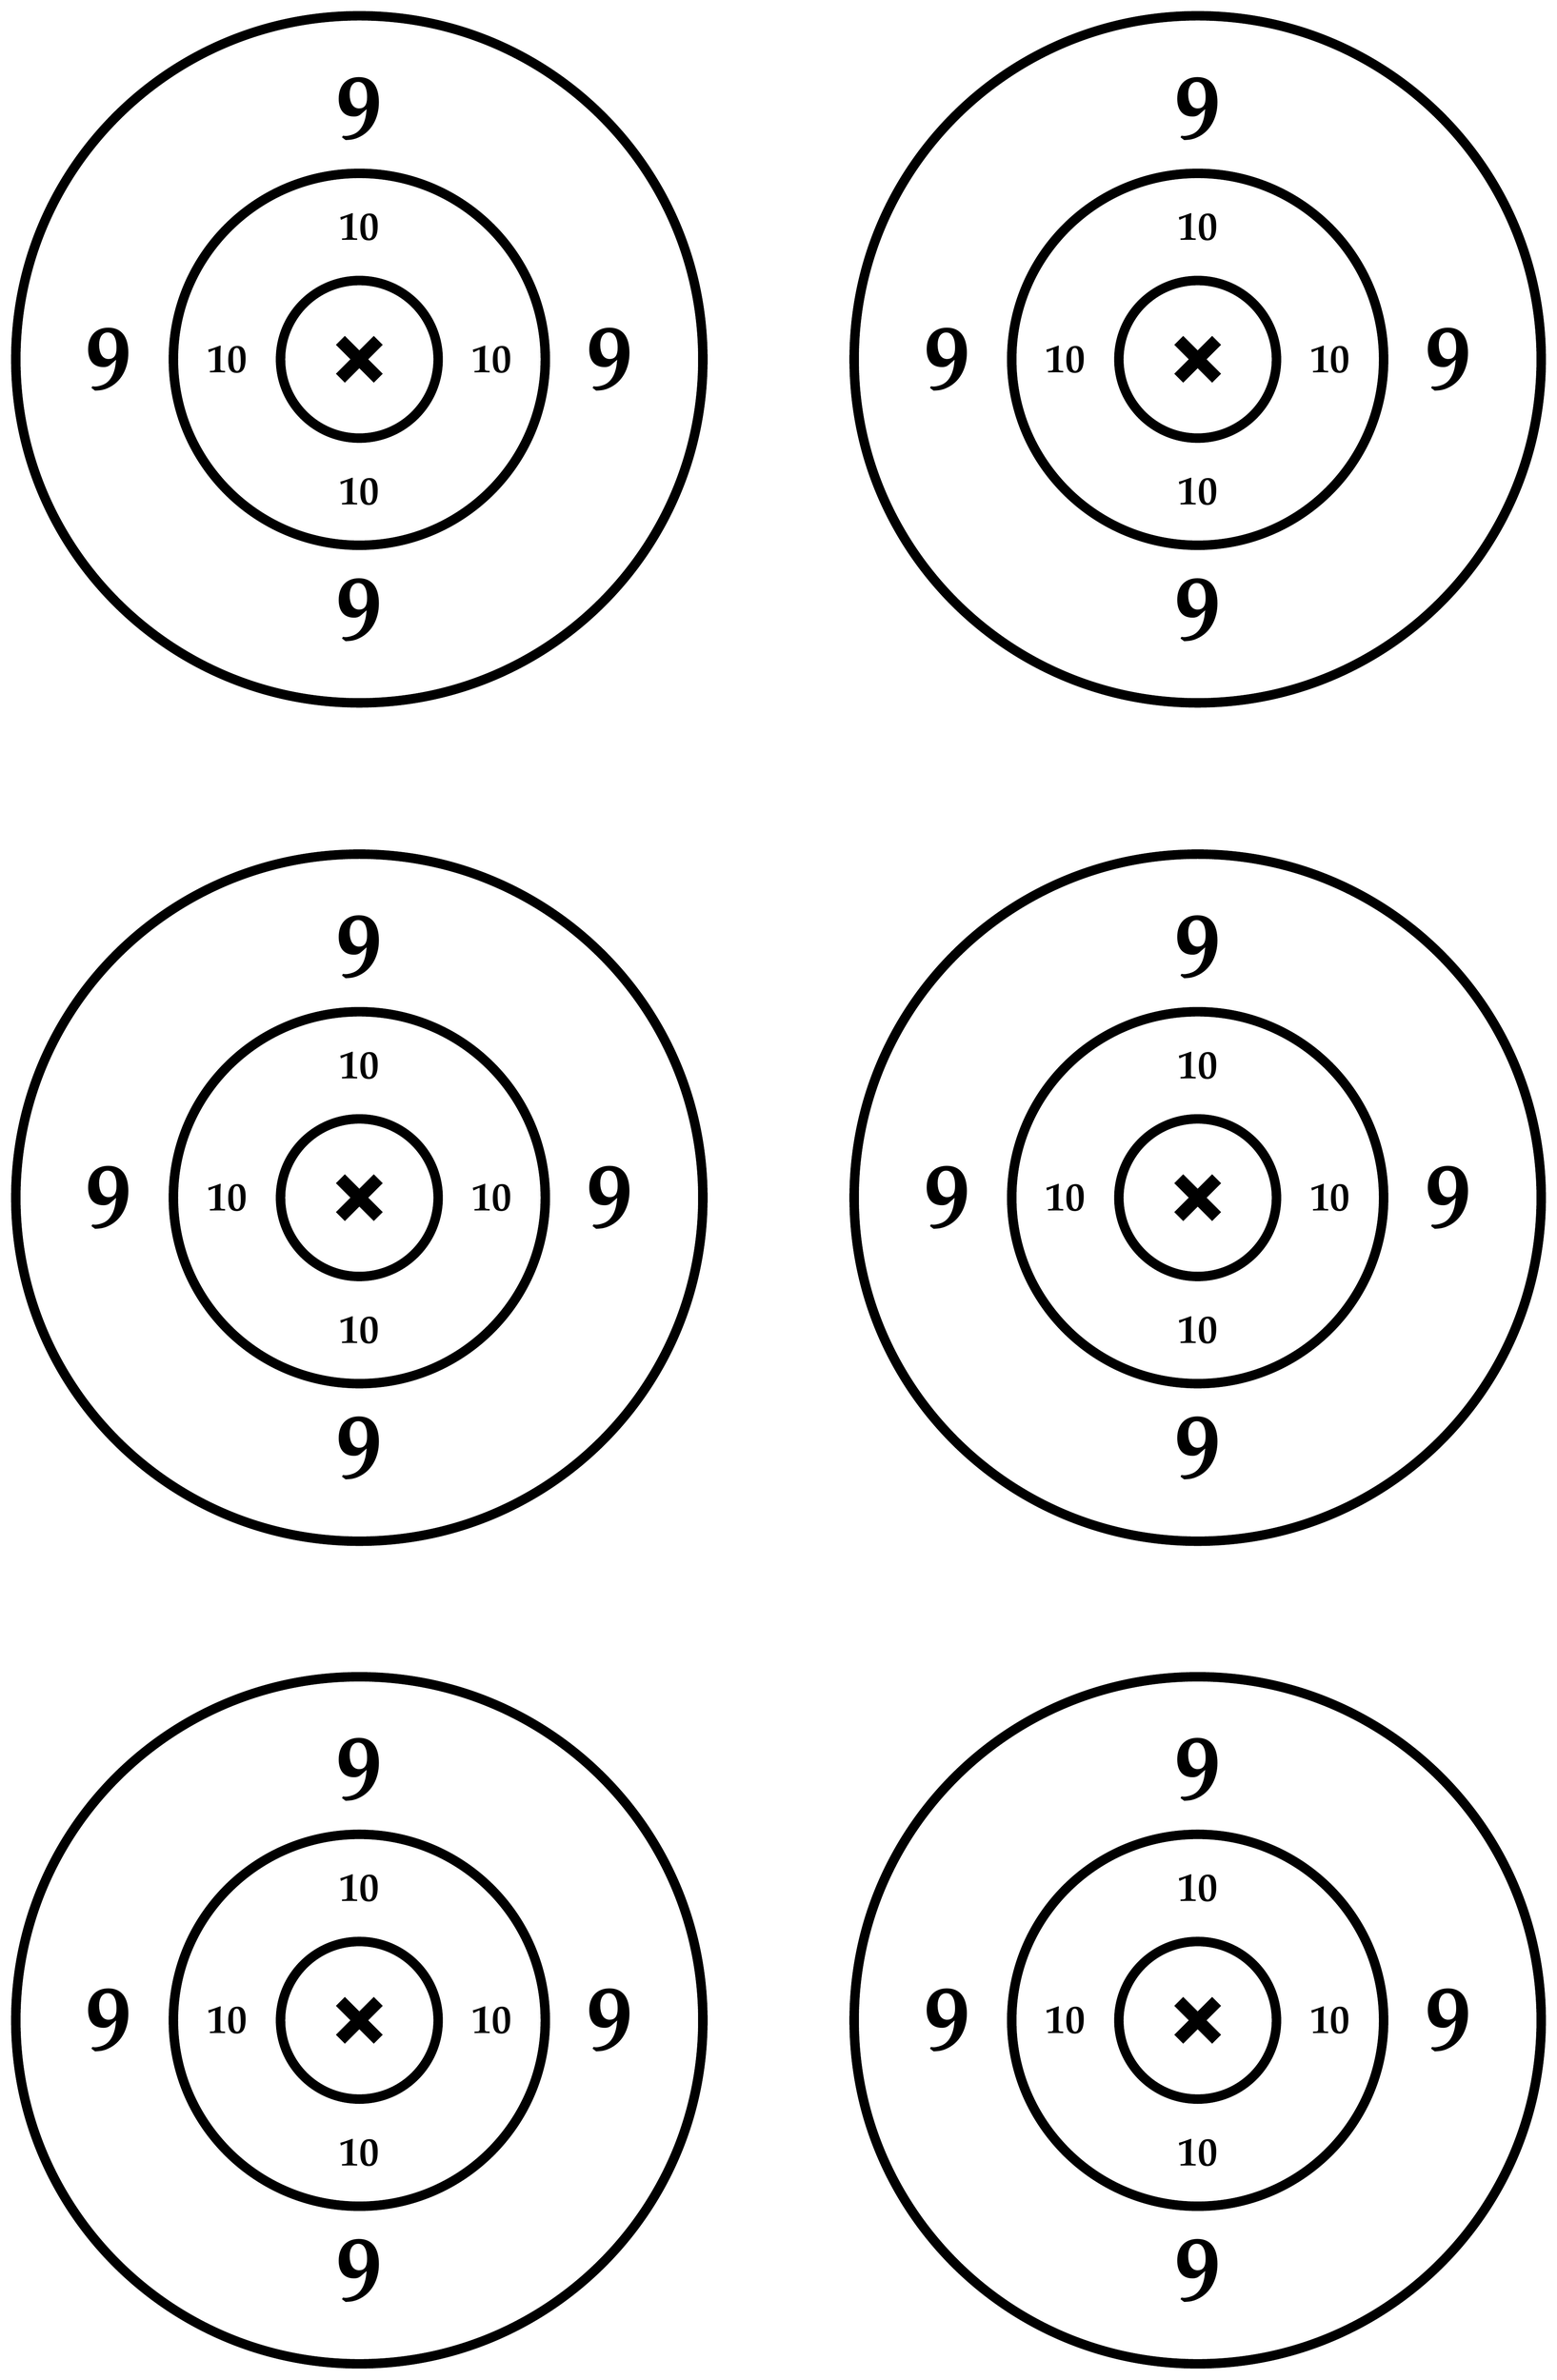
\begin{tikzpicture}
  \begin{scope}[shift={(00mm,5mm)}]
	  \pic at (30mm, 0mm) {300mT};
  \end{scope}
  \begin{scope}[shift={(296mm,5mm)}]
            \pic{300mT};
  \end{scope}
  \begin{scope}[shift={(0mm,266mm)}]
	  \pic at (30mm, 0mm) {300mT};
  \end{scope}
  \begin{scope}[shift={(296mm,266mm)}]
            \pic{300mT};
  \end{scope}

	\begin{scope}[shift={(0mm,532mm)}]
	  \pic at (30mm, 0mm) {300mT};
  \end{scope}
  \begin{scope}[shift={(296mm,532mm)}]
            \pic{300mT};
  \end{scope}
\end{tikzpicture}
\end{center}
\end{document}
